\documentclass[11pt]{article}

\usepackage{float}
\usepackage{hyperref}
\usepackage{enumerate}
\usepackage{graphicx}
\usepackage{amsmath}
\usepackage{epstopdf}
\usepackage{minted}
\usepackage{parskip}
\usepackage[toc,page]{appendix}
\usepackage{gensymb}
% formatting
\usepackage{fullpage}
\usepackage{verbatim}
\let\verbatiminput=\verbatimtabinput
\def\verbatimtabsize{4\relax}

\begin{document}
\title{EE 142 Lab 0 Report - Agilent ADS Introduction}

\author{Vighnesh Iyer}
\date{Monday, August 28, 2017}
\maketitle

\section{DC Simulation}
I setup a DC simulation to characterize the Predictive Transistor Model (PTM) BSIM4 MOSFET device. It's nominal supply is $V_{DD} = 0.9V$ and we sweep its $V_{DS}$ and $V_{GS}$ and record the drain current $I_{DS}$ reported by the model.

\subsection{$I_{ds}$ vs $V_{gs}$ and $I_{ds}$ vs $V_{ds}$}
\begin{figure}[H]
	\minipage{0.50\textwidth}
	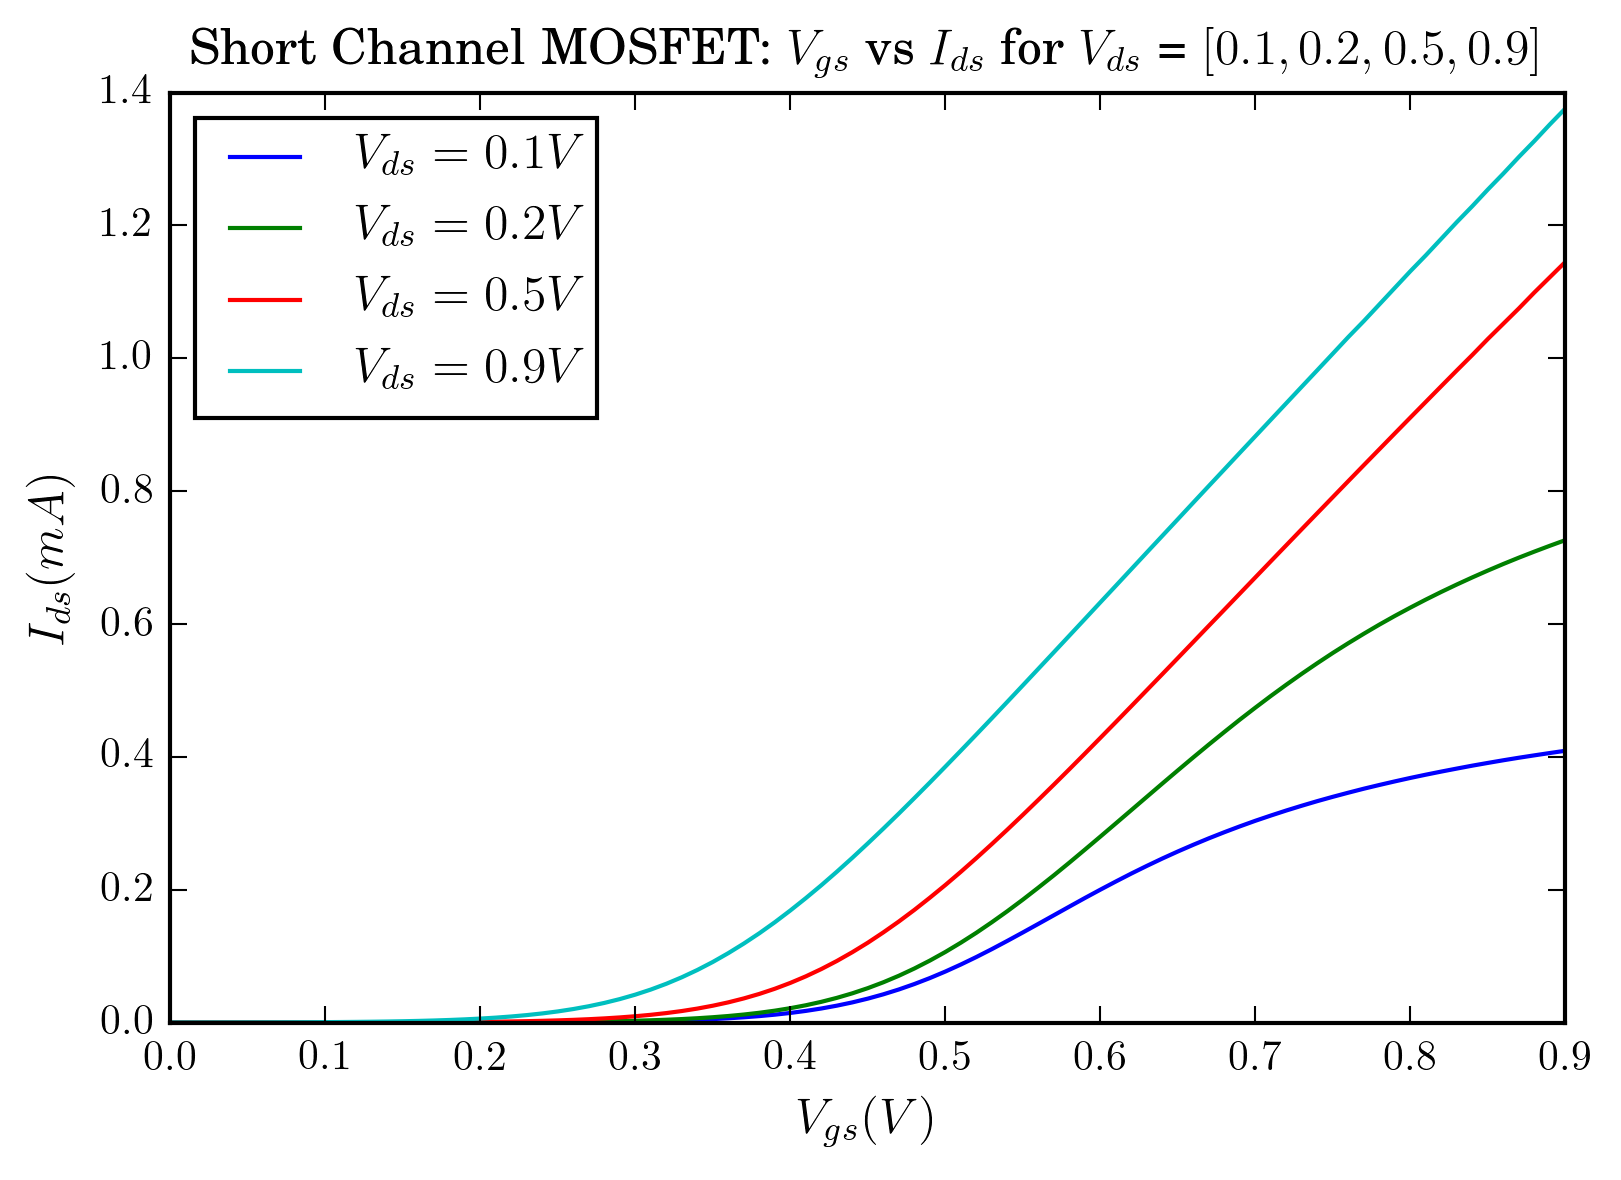
\includegraphics[width=\linewidth]{images/short_channel_vgs_vs_ids.png}
	\endminipage\hfill
	\minipage{0.50\textwidth}
	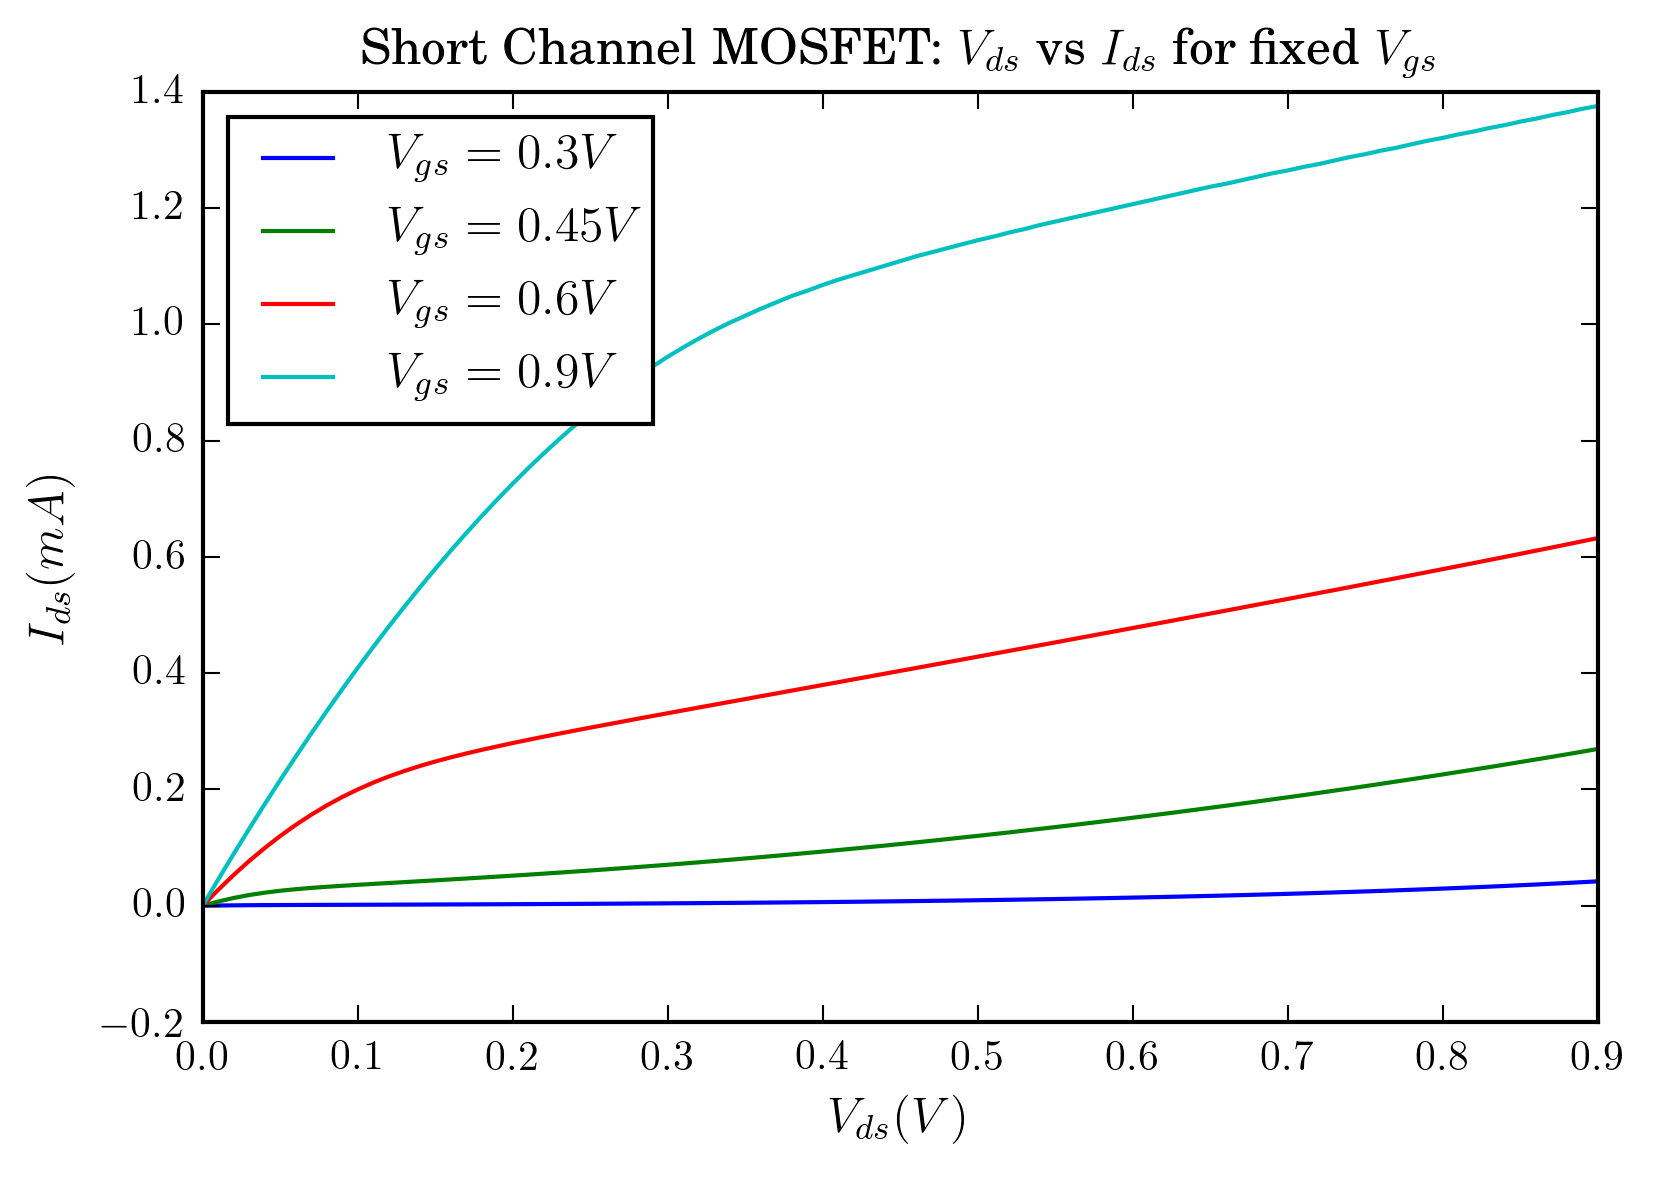
\includegraphics[width=\linewidth]{images/short_channel_vds_vs_ids.png}
	\endminipage
\end{figure}

\subsection{Long-Channel vs. Short-Channel MOSFETs}
I used the built-in/default Level 3 MOSFET model in ADS to represent a typical long-channel MOSFET model. Its I-V curves are plotted below.
\begin{figure}[H]
	\minipage{0.50\textwidth}
	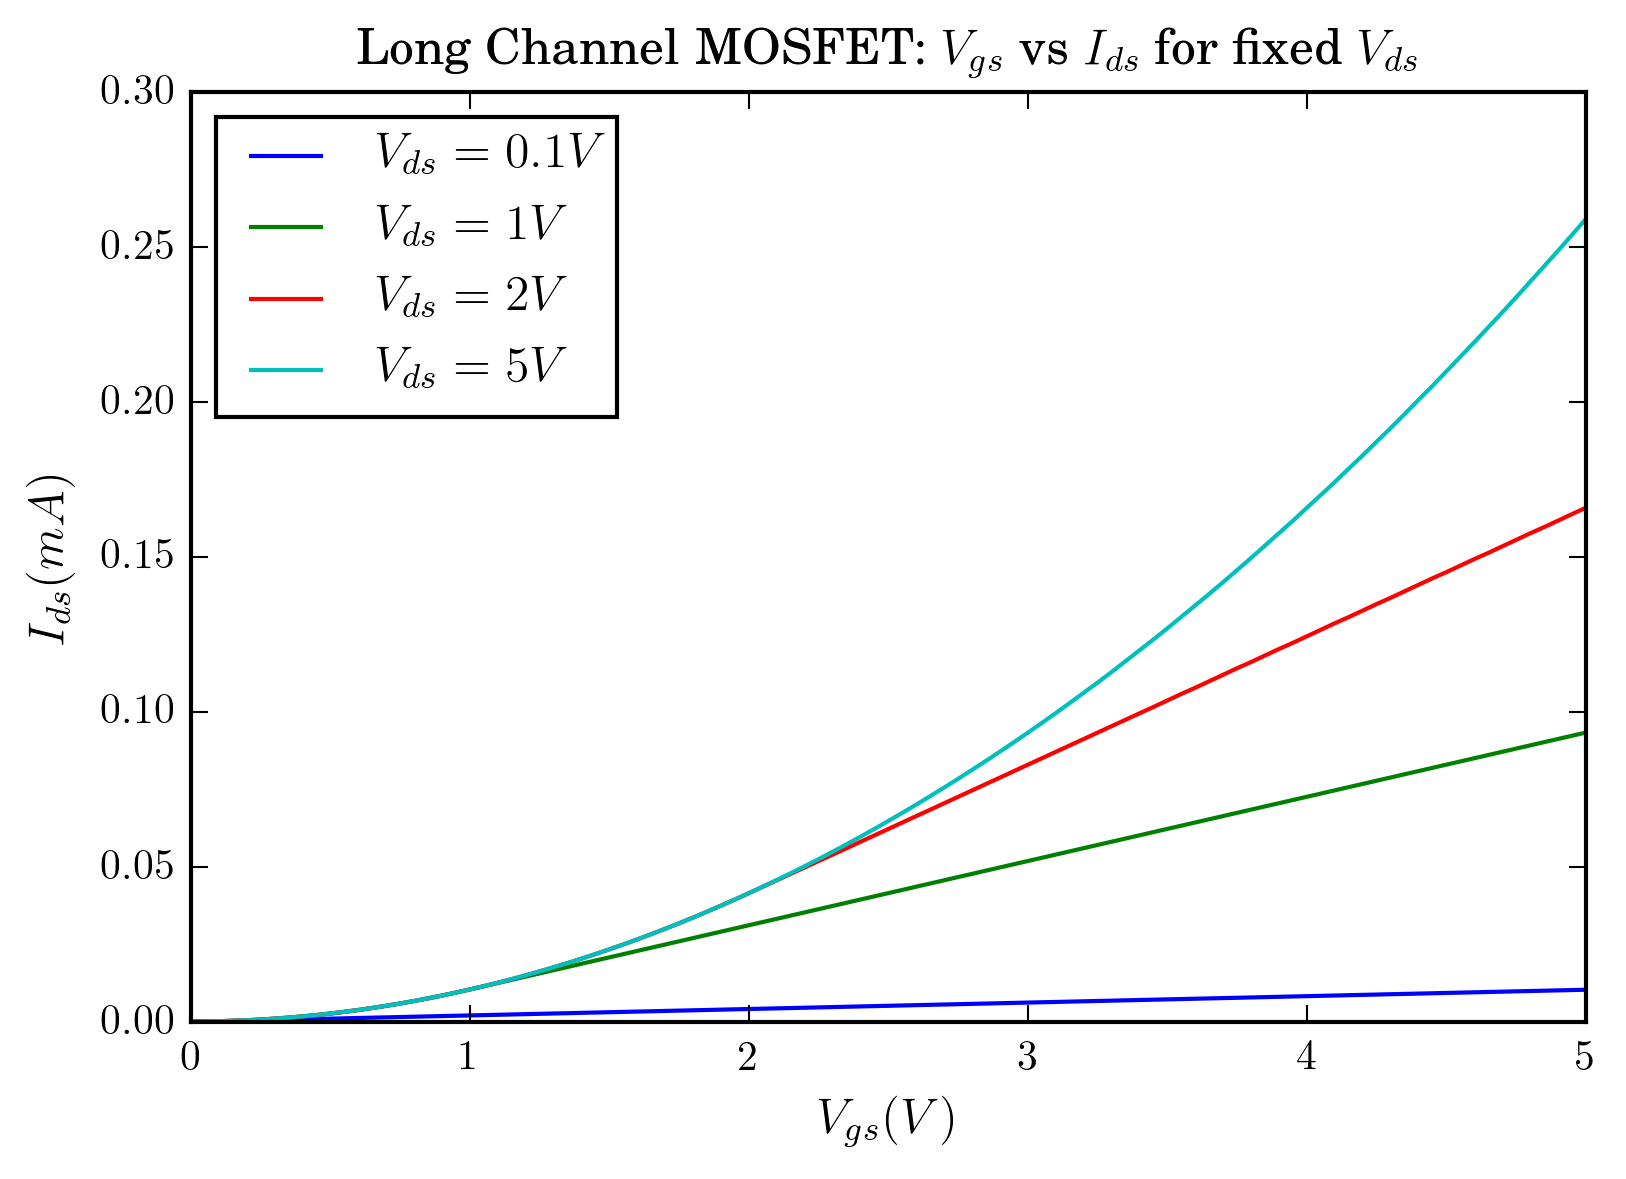
\includegraphics[width=\linewidth]{images/long_channel_vgs_vs_ids.png}
	\endminipage\hfill
	\minipage{0.50\textwidth}
	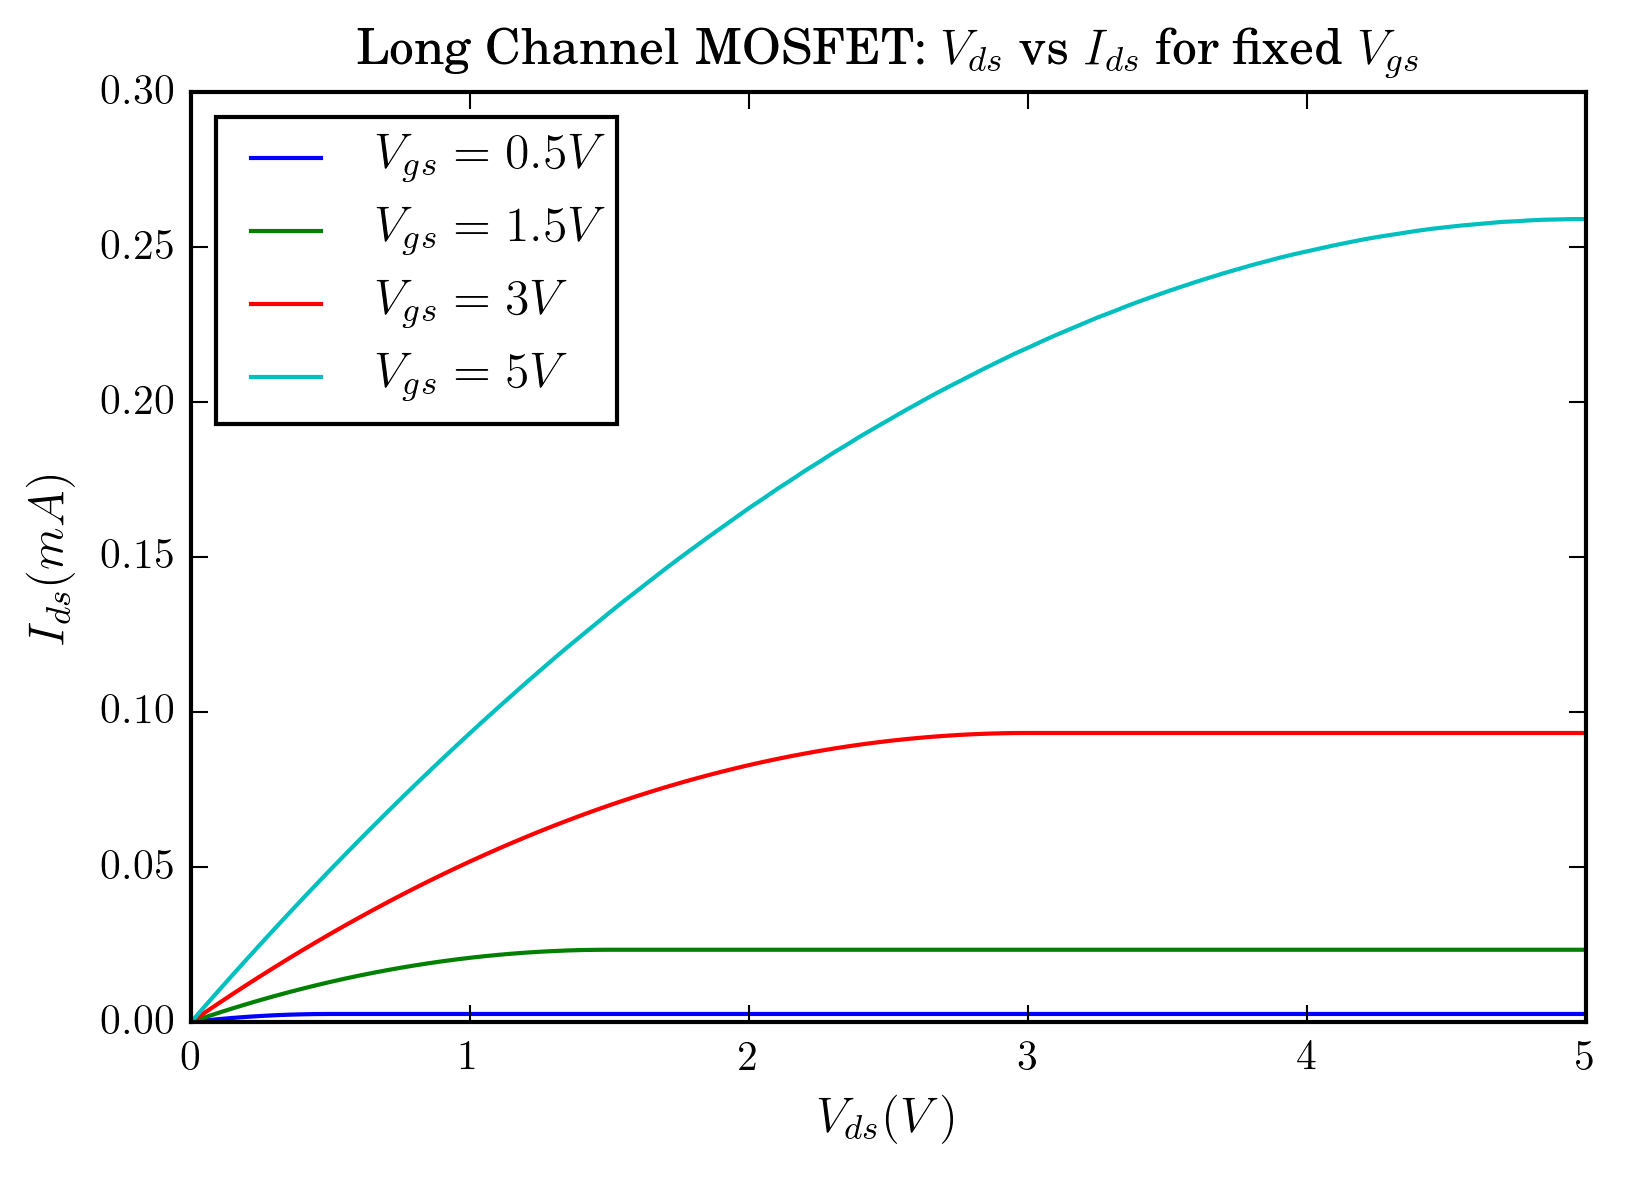
\includegraphics[width=\linewidth]{images/long_channel_vds_vs_ids.png}
	\endminipage
\end{figure}

We can see some major differences in the shape of the curves, which can be explained by various short-channel effects:

\begin{itemize}
	\item DIBL (drain induced barrier lowering)
	
	DIBL is a short-channel phenomenon where the threshold voltage of the transistor is reduced as $V_{DS}$ increases. This can be easily seen in the first plot where larger $V_{DS}$ values lead to a significantly smaller value of $V_{th}$ when extrapolated from the plot's linear region. This isn't the case for the long-channel MOSFET model where the extrapolated $V_{th}$ values are very close for a large variation in $V_{DS}$.
	
	This effect is particularly pronounced when operating in the subthreshold region, where the DIBL effect can lead to significantly higher subthreshold (leakage) currents, and compromise the power efficiency of smaller transistors.

	\item Channel Length Modulation (similar to BJT early effect)
	
	The effect of channel length modulation can be modeled like:
	
	\begin{equation*}
		I_{DS} = I_{DS, nominal} \cdot (1 + \lambda V_{DS}) 
	\end{equation*} 
	
	which means that the effective channel length of the FET is affected by $V_{DS}$. This can be seen by comparing plots 2 and 4, where for the long-channel device, after reaching the point of $V_{DS} = V_{ov}$ the curve flattens out to nearly horizontal, while for the short-channel device, the curve has a positive slope. One effect of channel length modulation is to reduce the small-signal $r_o$ and thereby reduce the FET's small-signal gain.
	
	\item Velocity Saturation
	
	A short-channel MOSFET's carrier velocity is proportional to the strength of the electric field caused by the voltage applied at the gate relative to the source up until a particular point, where the charge carriers can't move any faster. This limits the actual current below the current predicted by the quadratic law for saturation region operation.
	
	We can see this effect in plots 2 and 4, where for a long-channel device the drain current scales quadratically with $V_{GS}$ but for the short-channel device, the drain current scales linearly with $V_{GS}$ in the saturation region.
\end{itemize}

\section{AC Simulation}
\subsection{MOSFET Transconductance $g_m$}
We can measure $g_m$ versus the $V_{GS}$ and $V_{DS}$ DC bias points:

\begin{equation*}
	g_m = \frac{i_{ds}}{v_{gs}}
\end{equation*}

where $i_{ds}$ is the AC small signal drain current and $v_{gs}$ is the AC small signal gate voltage, which is fixed at 10 mV for this simulation.

We run an AC simulation several times, with the frequency fixed at 10 MHz and sweeping the DC bias points of $V_{GS}$ and $V_{DS}$ from 0 to 0.9 V. The $v_{gs}$ AC magnitude is 10 mV. The following plots can be derived:

\begin{figure}[H]
	\minipage{0.50\textwidth}
	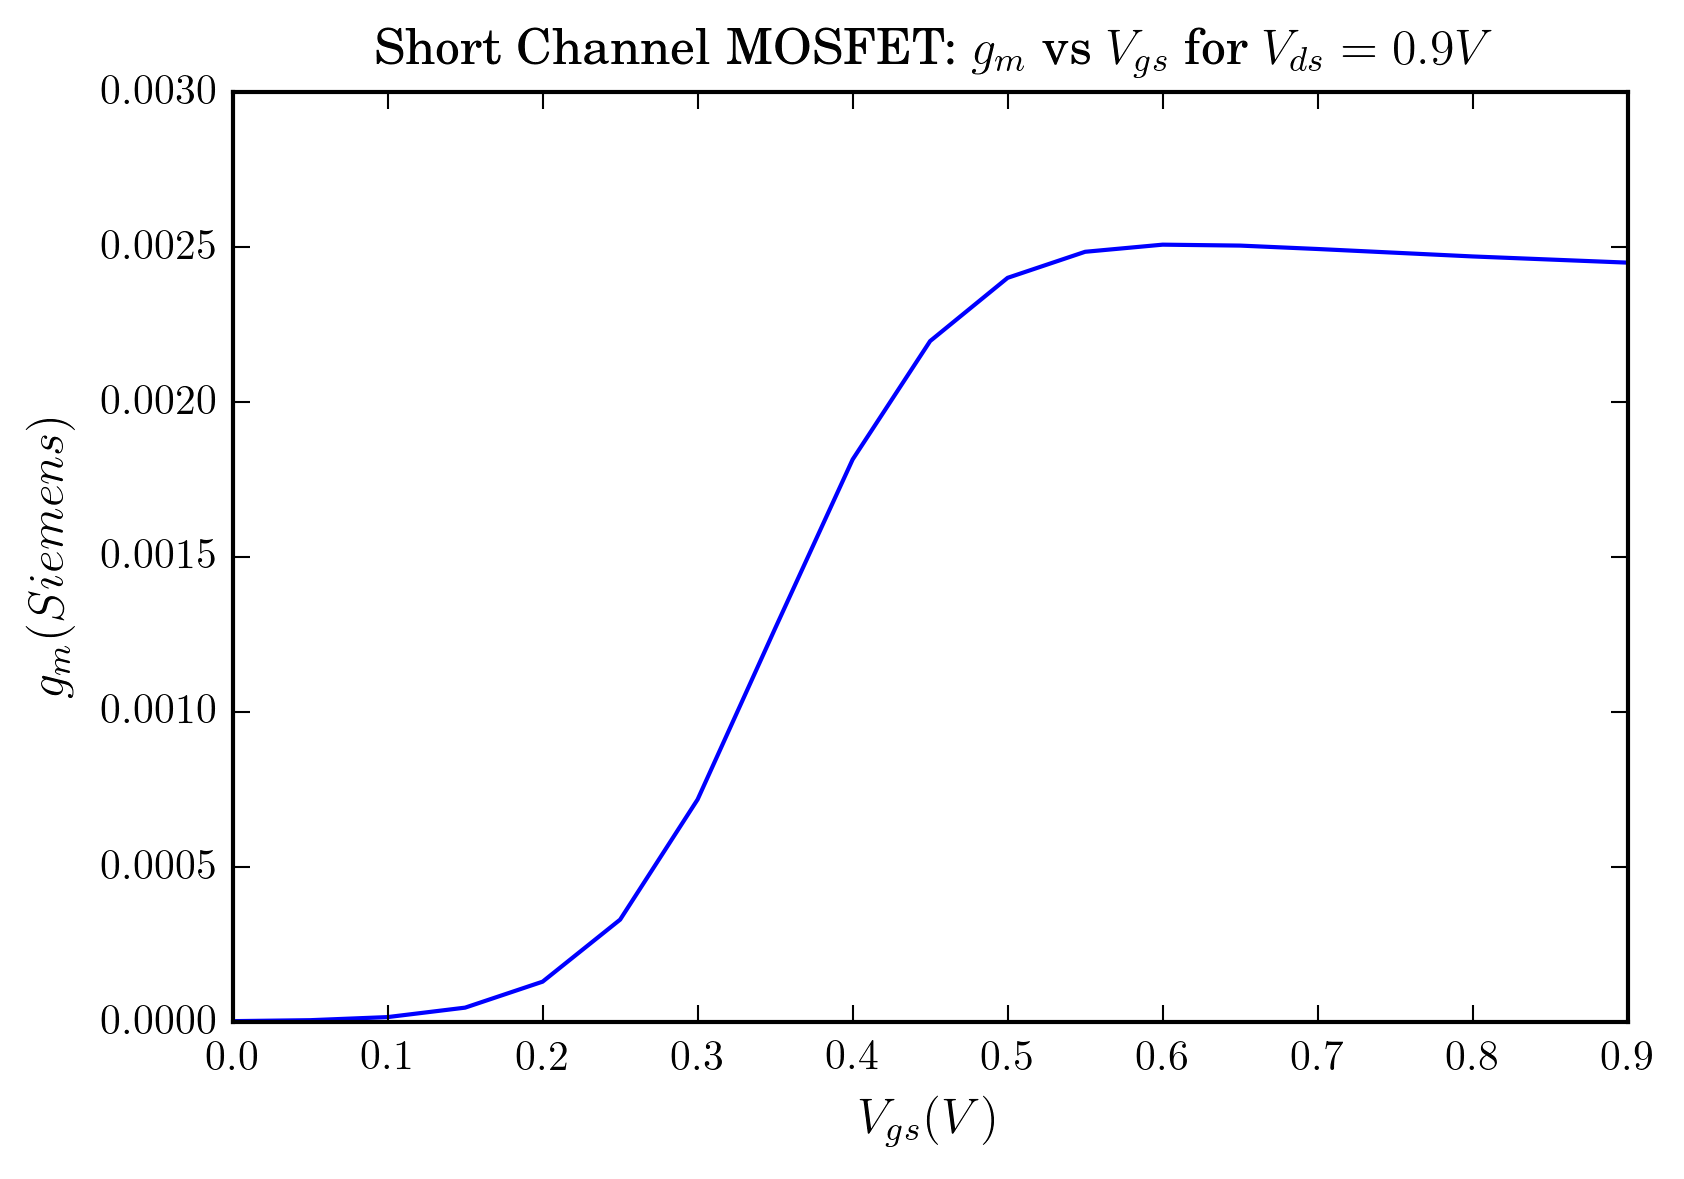
\includegraphics[width=\linewidth]{images/short_channel_gm_vs_vgs.png}
	\endminipage\hfill
	\minipage{0.50\textwidth}
	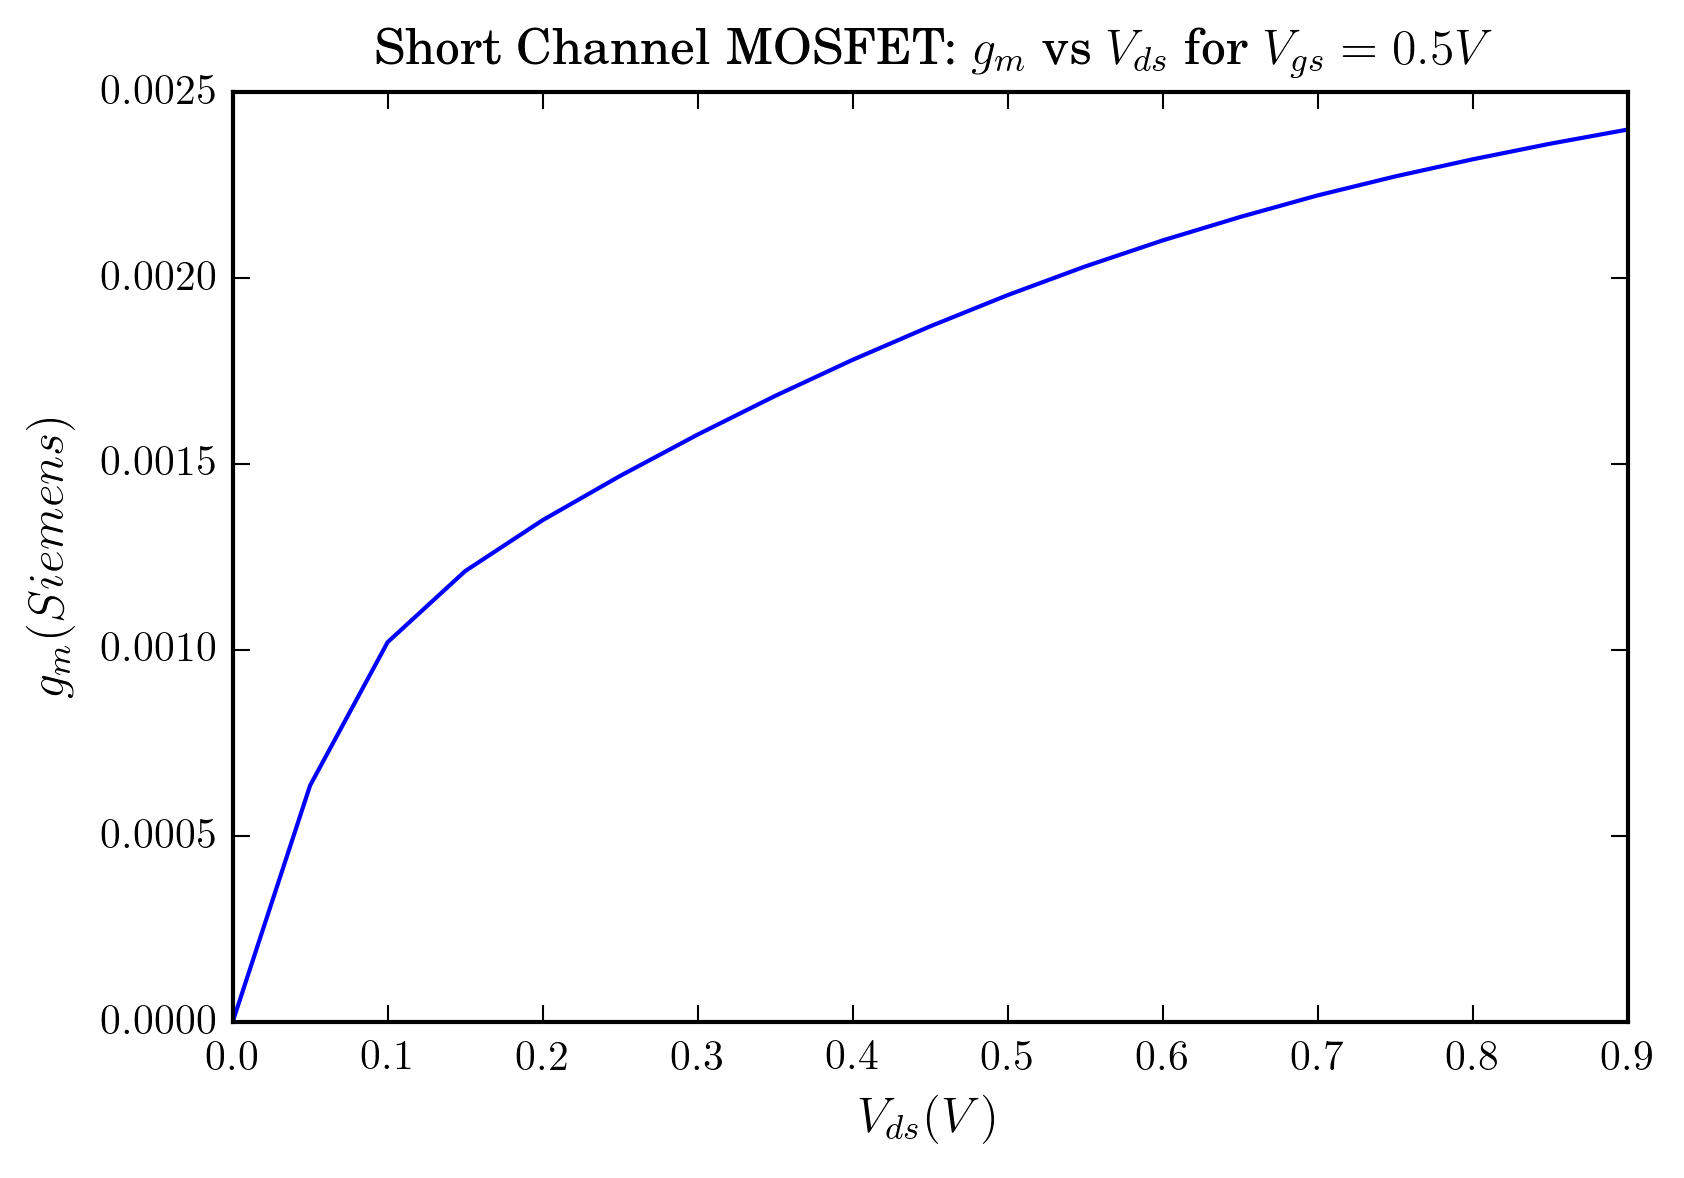
\includegraphics[width=\linewidth]{images/short_channel_gm_vs_vds.png}
	\endminipage
\end{figure}

For a fixed $V_{DS}$, as $V_{GS}$ increases from 0V, the transconductance goes up until it saturates around 2.5mS; this translates to the MOSFET moving from the linear to the saturation region of operation. For a fixed $V_{GS}$, as $V_{DS}$ increases from 0V, the transconductance keeps increasing, although with a lower slope with higher values of $V_{DS}$. 

\subsection{MOSFET Output Resistance $r_o$ and Voltage Gain $A_v$}
We can measure $r_o$ versus $V_{DS}$ DC bias points:

\begin{eqnarray}
	r_o = \frac{v_{ds}}{i_{ds}} \nonumber \\
	|A_V| = g_m r_o \nonumber
\end{eqnarray}

by holding $V_{GS}$ at 0.5 VDC, and applying a AC voltage source with magnitude 10 mV at the drain. The following plots can be derived:

\begin{figure}[H]
	\minipage{0.50\textwidth}
	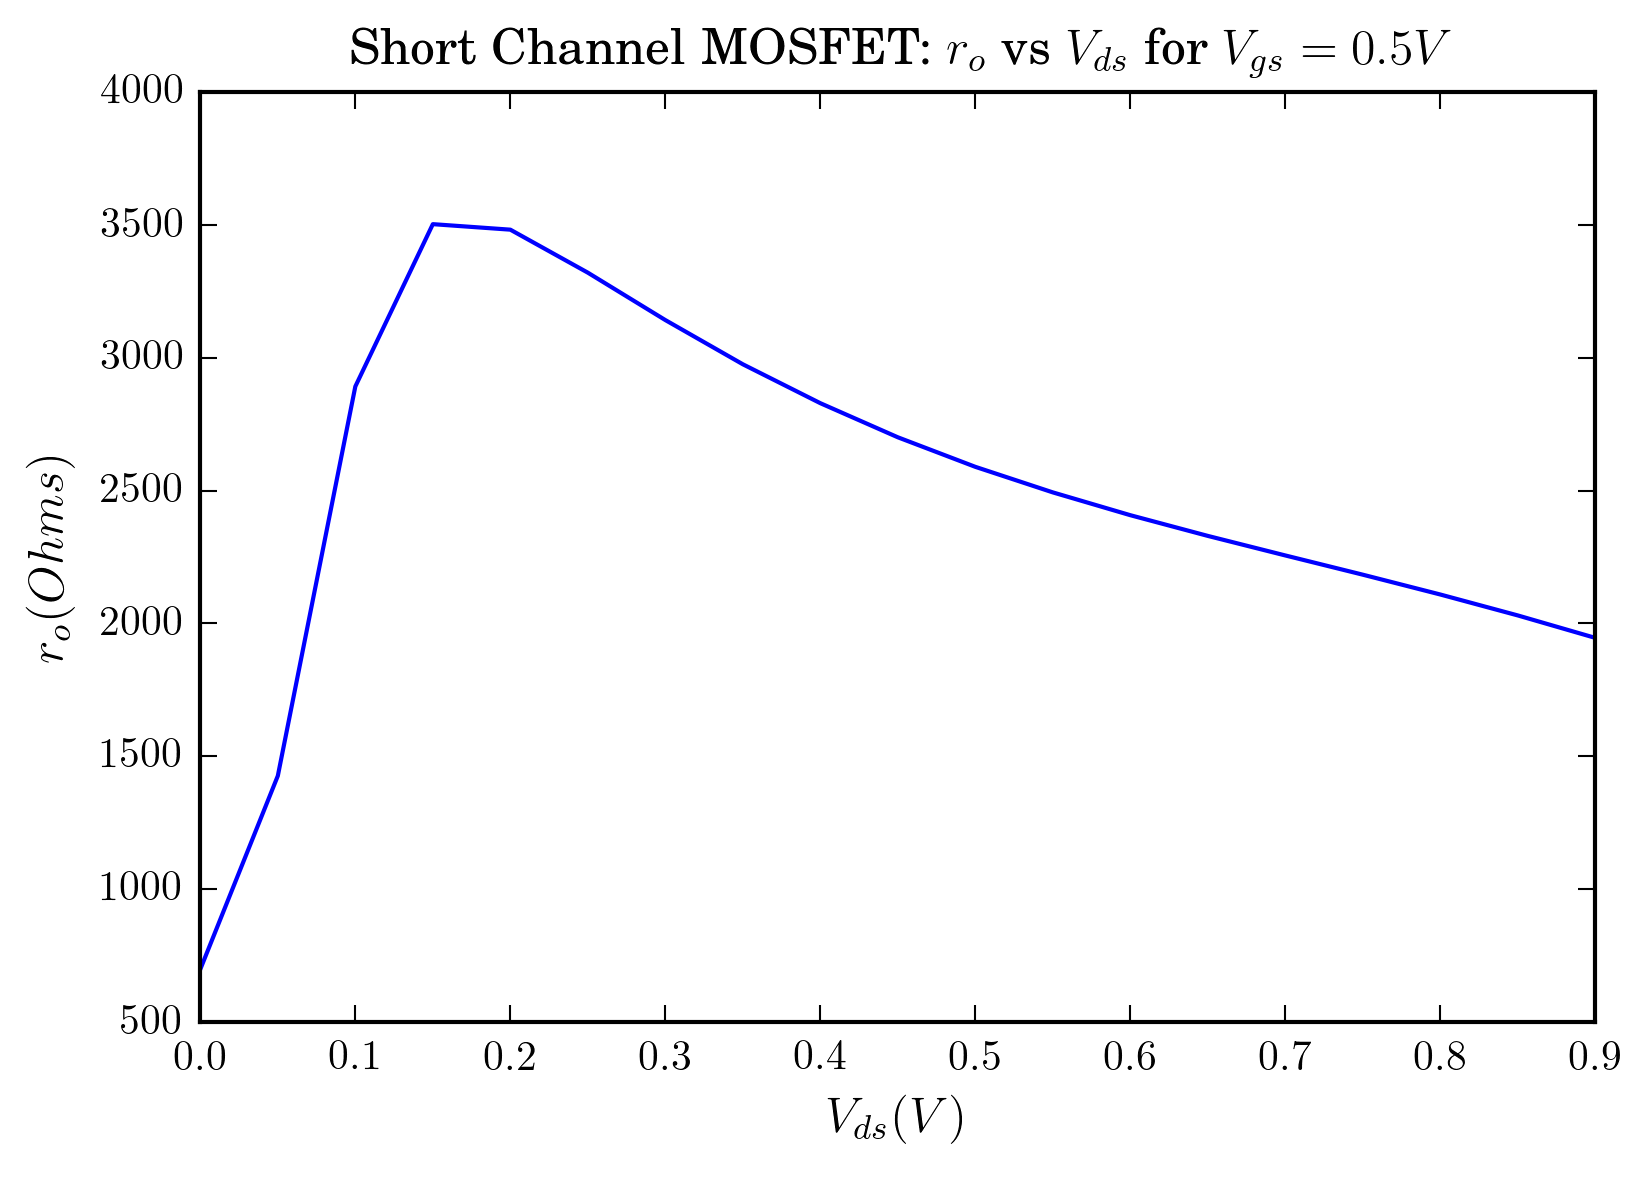
\includegraphics[width=\linewidth]{images/short_channel_ro_vs_vds.png}
	\endminipage\hfill
	\minipage{0.50\textwidth}
	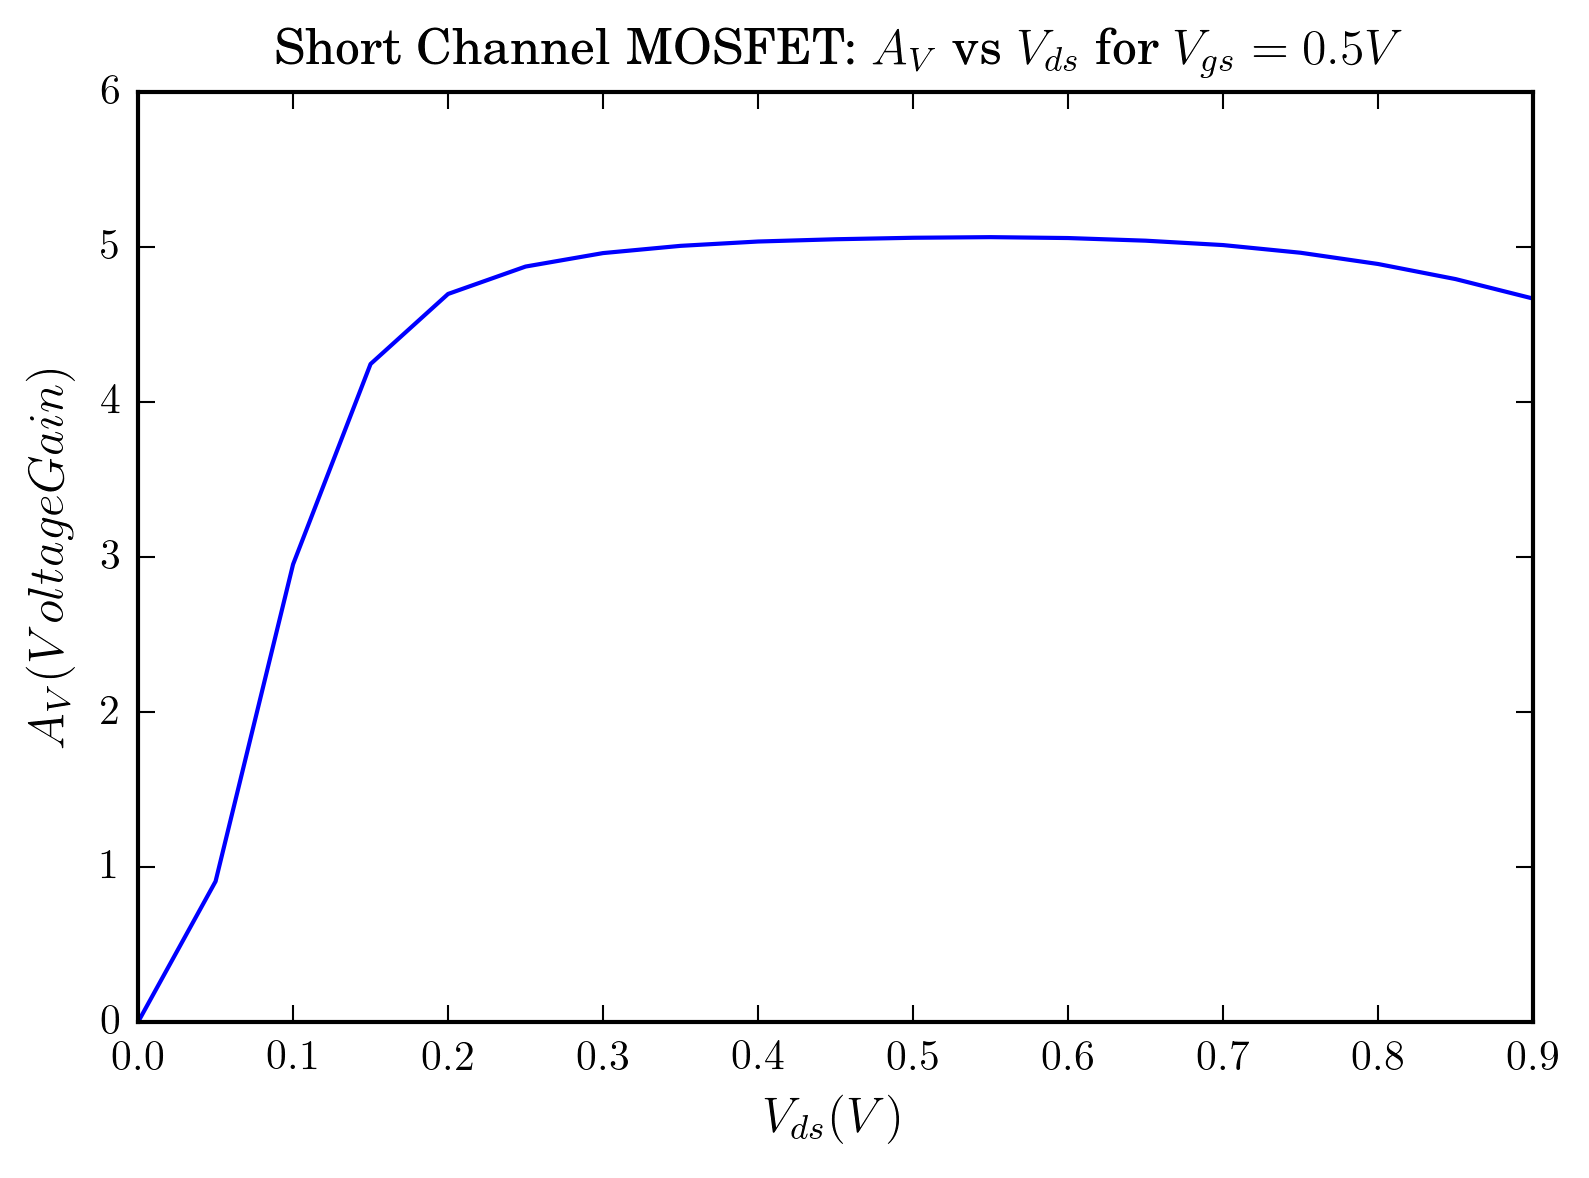
\includegraphics[width=\linewidth]{images/short_channel_av_vs_vds.png}
	\endminipage
\end{figure}

We can see that $r_o$ spikes to its highest value when $V_{DS} \approx V_{ov}$ and then decreases slowly as the MOSFET moves further into saturation. Since this follows the opposite trend of $g_m$, the gain is relatively stable around 5 V/V once the MOSFET is firmly in saturation and properly biased.

\subsection{Long-Channel MOSFET Differences}
\begin{figure}[H]
	\minipage{0.50\textwidth}
	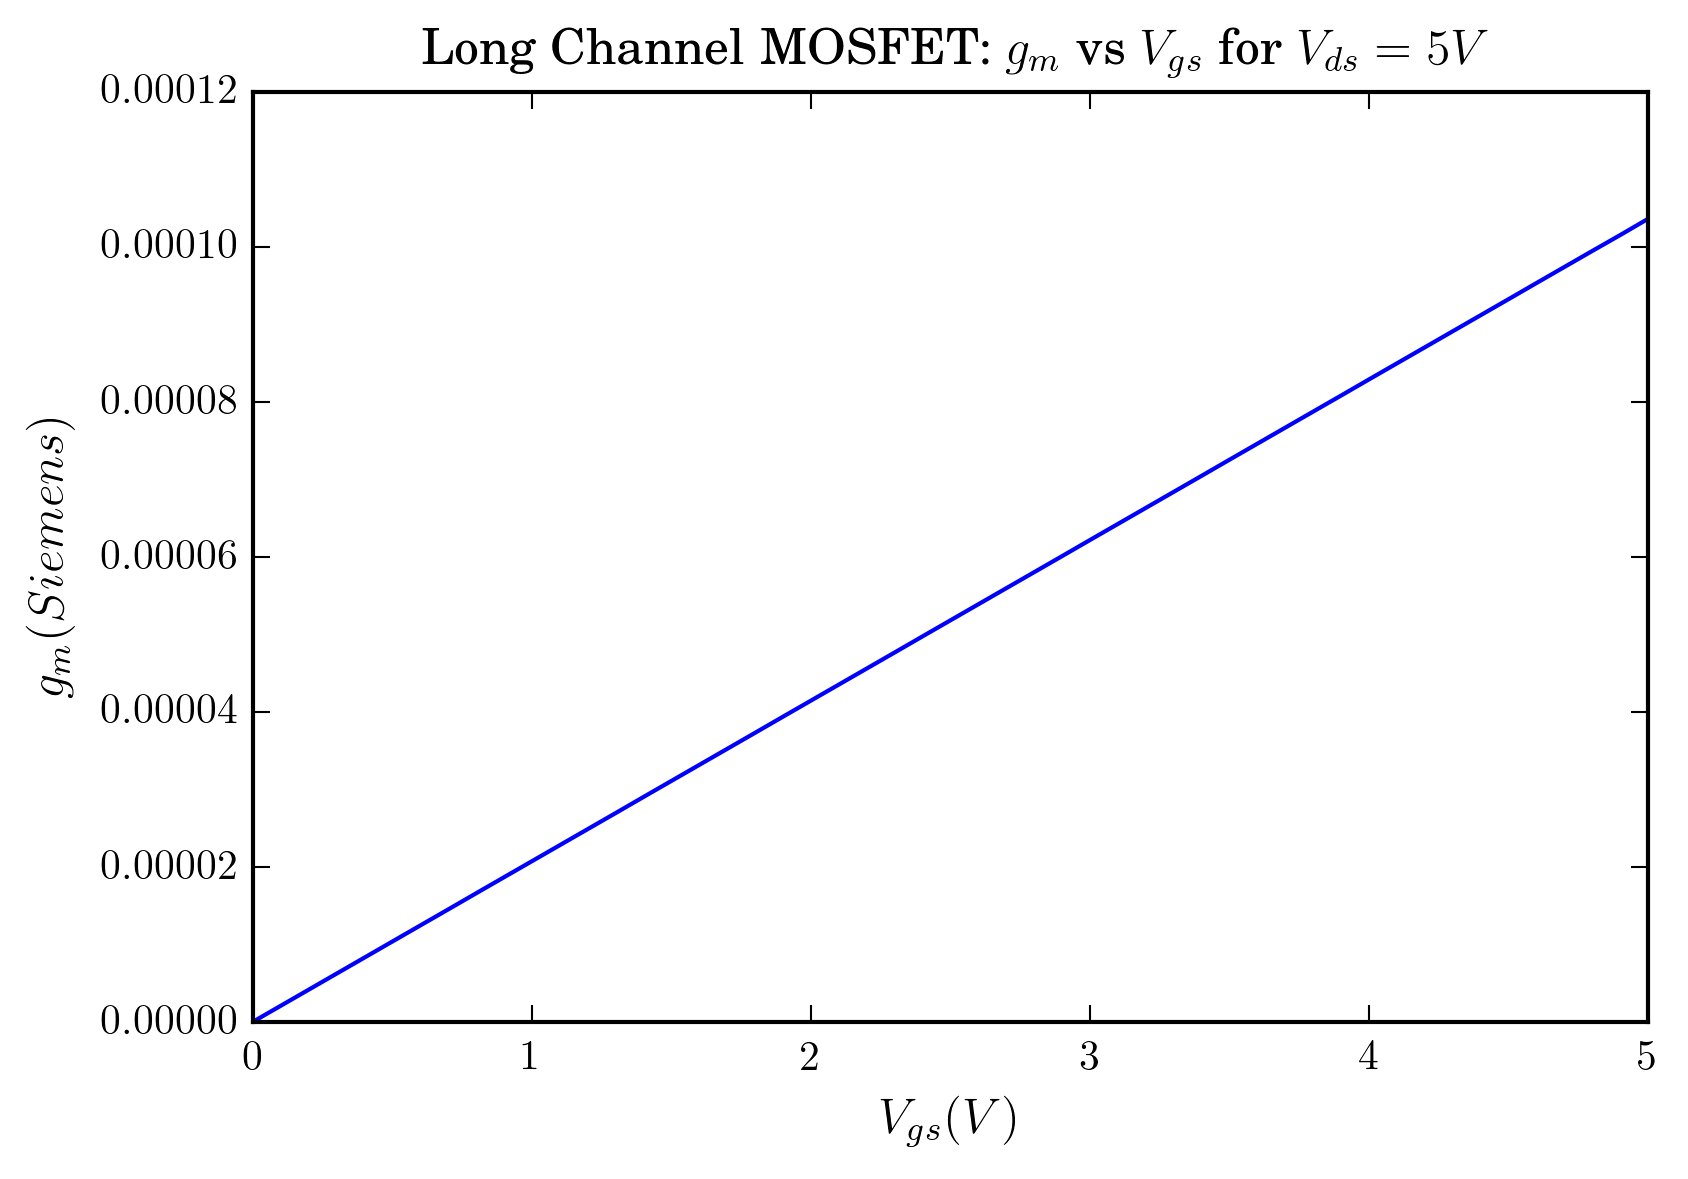
\includegraphics[width=\linewidth]{images/long_channel_gm_vs_vgs.png}
	\endminipage\hfill
	\minipage{0.50\textwidth}
	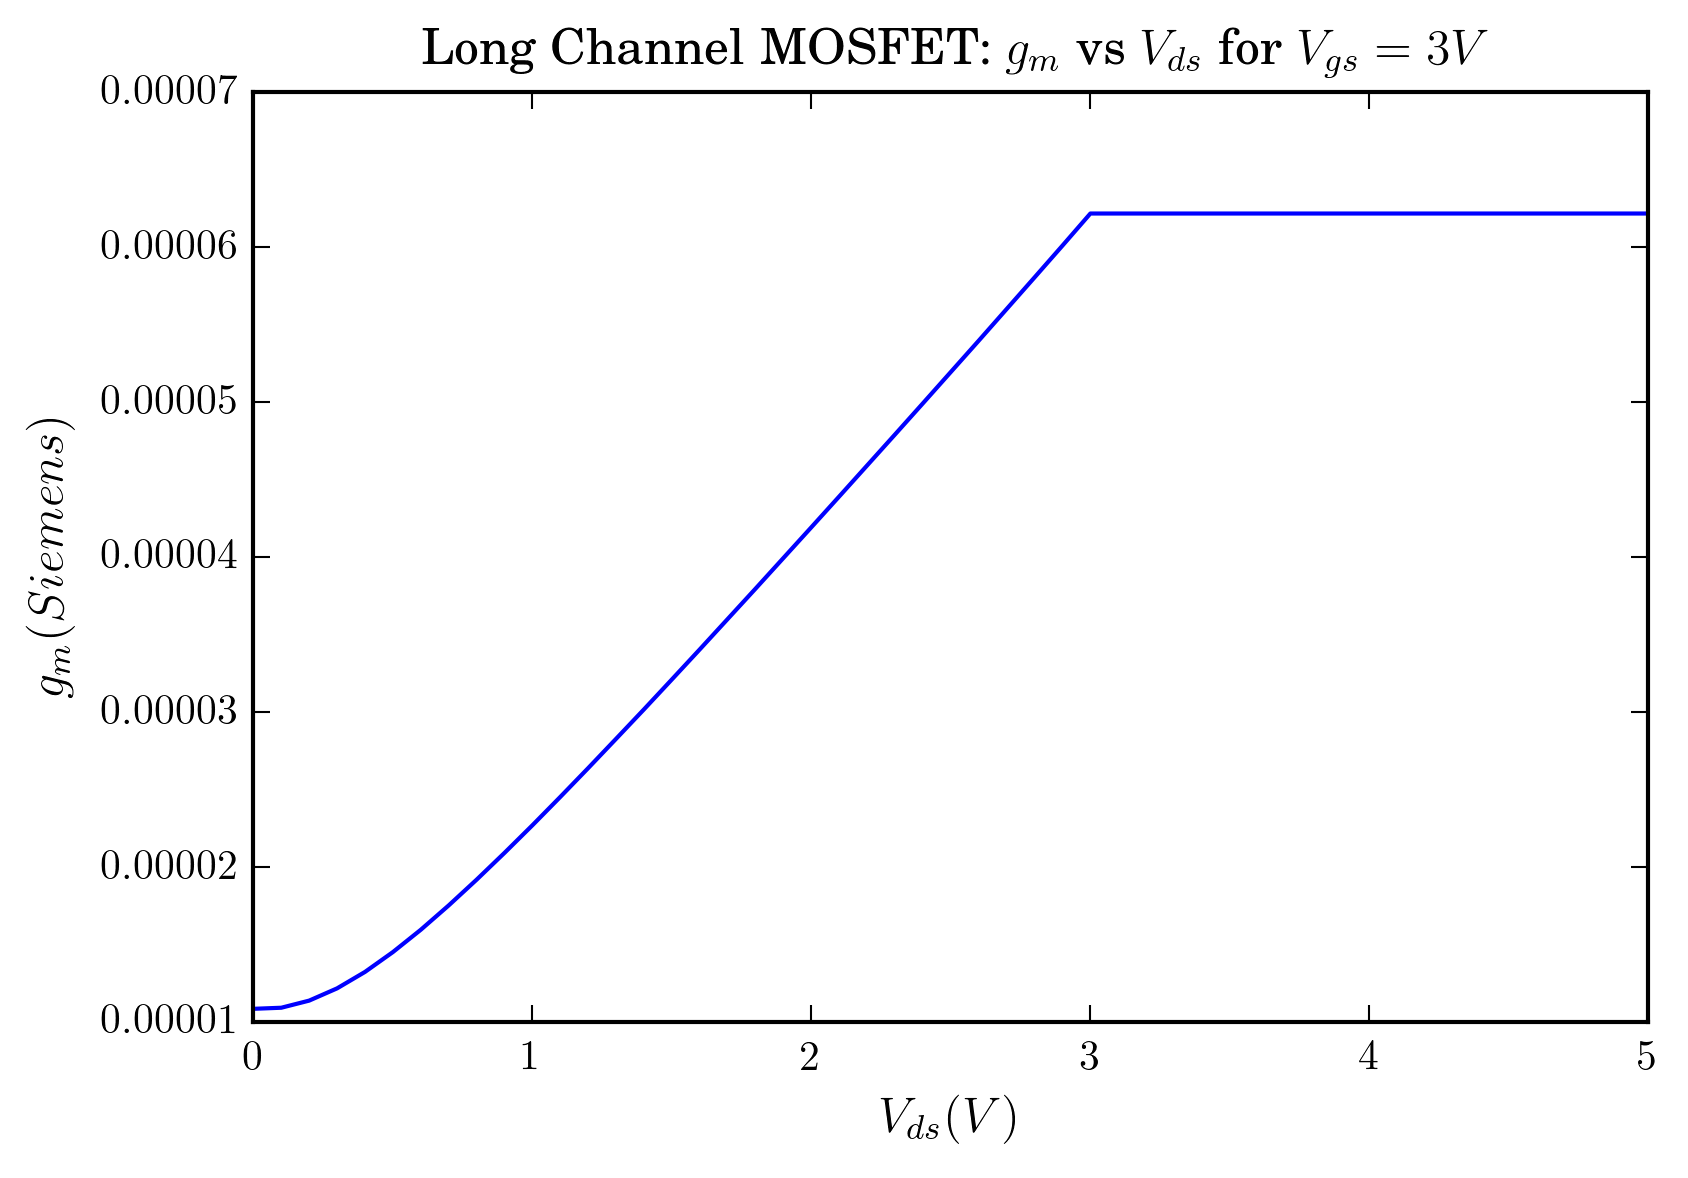
\includegraphics[width=\linewidth]{images/long_channel_gm_vs_vds.png}
	\endminipage
\end{figure}

\begin{figure}[H]
	\minipage{0.50\textwidth}
	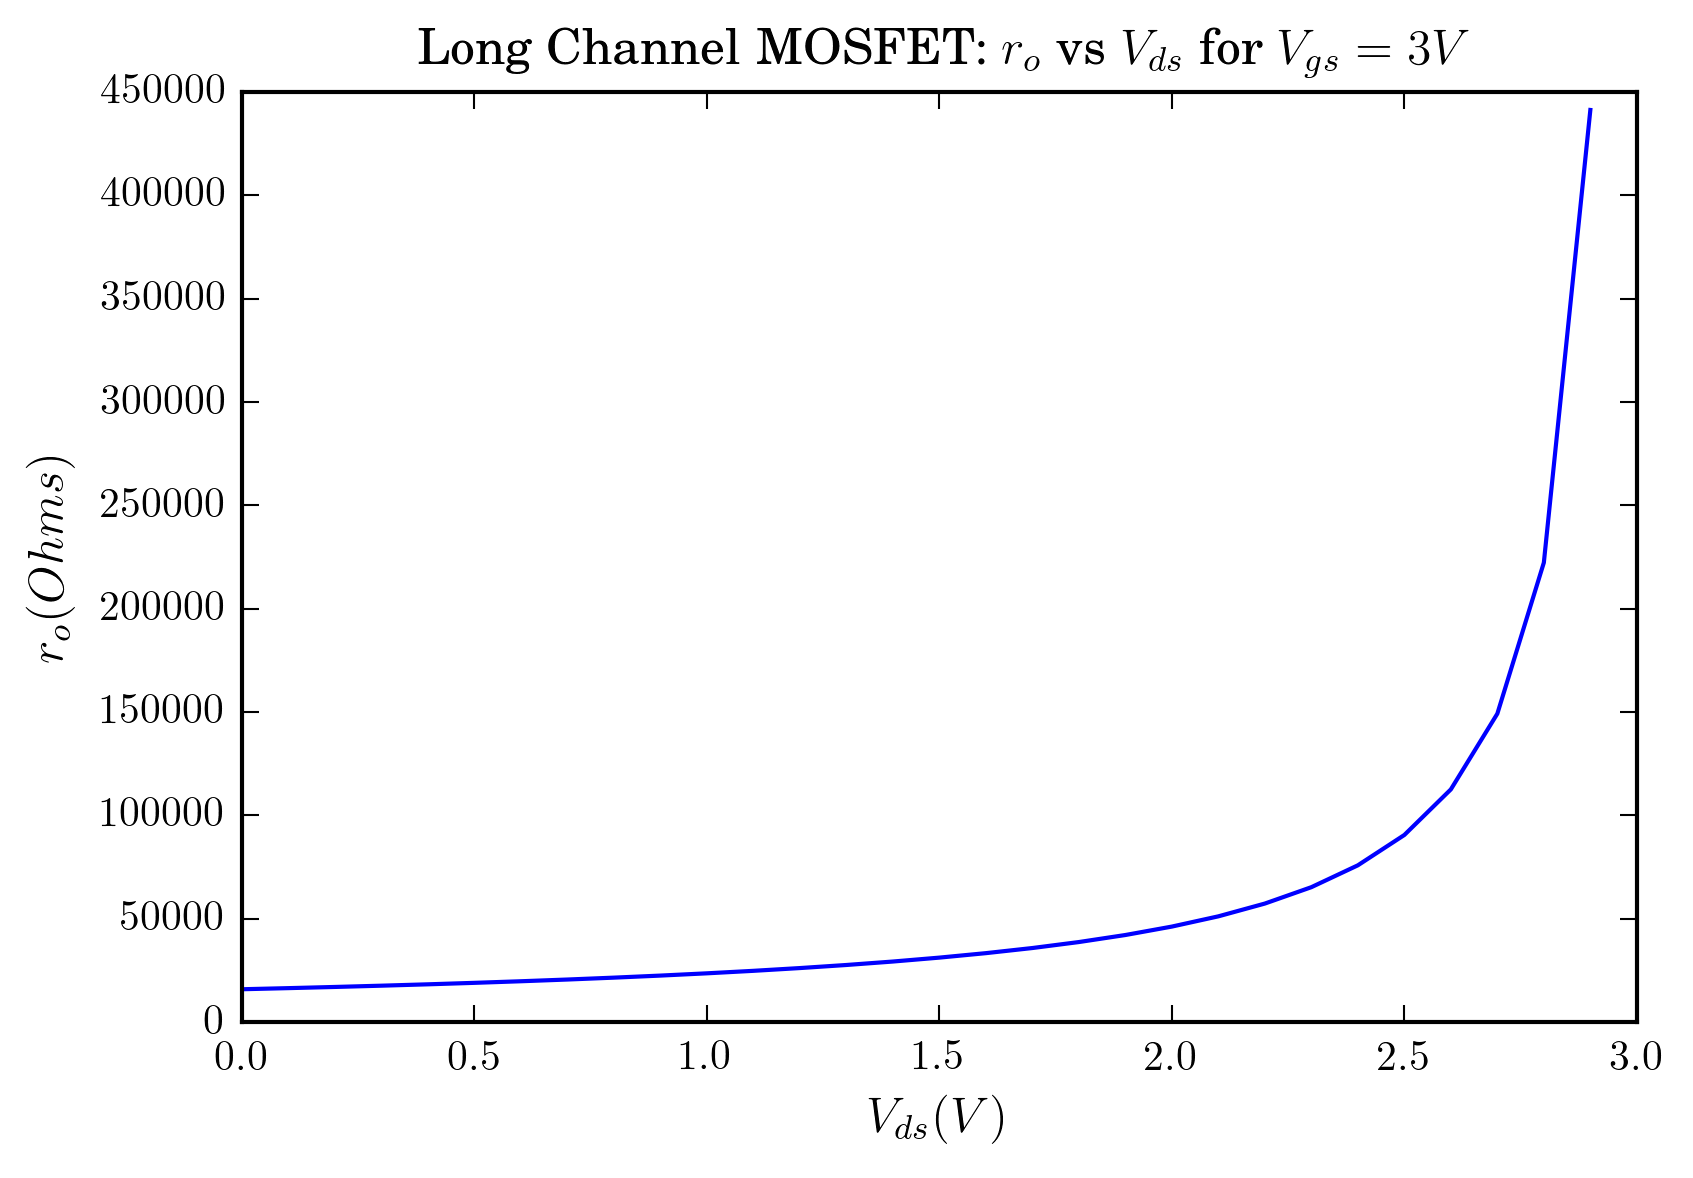
\includegraphics[width=\linewidth]{images/long_channel_ro_vs_vds.png}
	\endminipage\hfill
	\minipage{0.50\textwidth}
	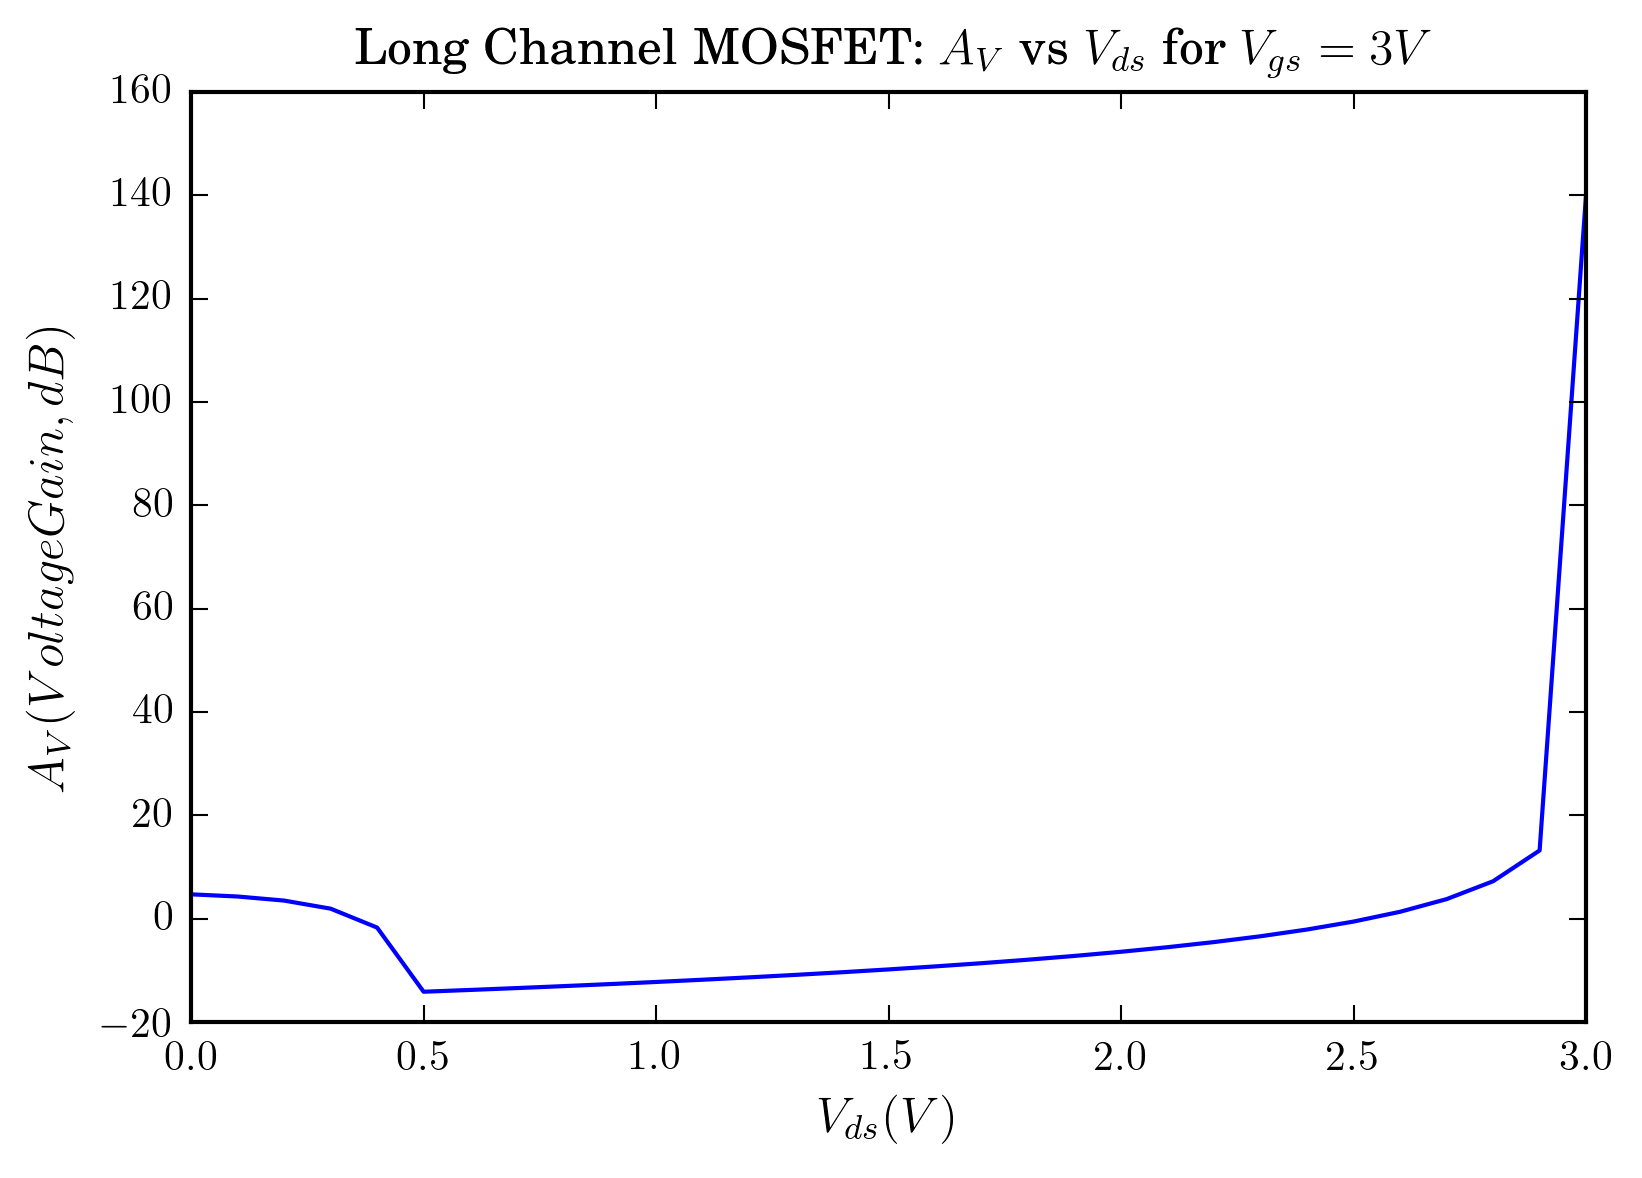
\includegraphics[width=\linewidth]{images/long_channel_av_vs_vds.png}
	\endminipage
\end{figure}

For a long-channel device, the $g_m$ curves are much more linear, and we don't see saturation effects. The $r_o$ curves look odd however, and the voltage gain seems to spike to infinity once $V_{DS} \geq V_{GS}$ which likely indicates some issue in the model I am using (there is a discontinuity somewhere).

Nevertheless, the overall difference of using a long-channel device is better (more linear) transconductance and output resistance (and voltage gain) compared to a short-channel device while having worse high frequency performance due to larger parasitic capacitances.

\end{document}